\subsection{二阶行列式}
\subsubsection{二元线性方程组}
\paragraph{}
用消元法解二元线性方程组
\begin{align}
\label{消元法解二元线性方程组}
\begin{split}
  \left\{ \begin{array}{l}
    a_{11}x_1 + a_{12}x_2 = b_1, \\
    a_{21}x_1 + a_{22}x_2 = b_2.
  \end{array} \right.
\end{split}
\end{align}

\paragraph{}
为消去未知数$x_2$,以$a_{22}$与$a_{12}$分别乘上列两方程的两端,然后两个方程相减,得
\begin{equation*}
  (a_{11}a_{22} - a_{12}a_{21})x_1 = b_1a_{22} - a_{12}b_2;
\end{equation*}
类似地,消去$x_1$,得
\begin{equation*}
  (a_{11}a_{22} - a_{12}a_{21})x_2 = a_{11}b_2 - b_1a_{21}.
\end{equation*}

\paragraph{}
当$a_{11}a_{22} - a_{12}a_{21} \neq 0$时,求得方程组\eqref{消元法解二元线性方程组}的解为
\begin{equation}
  \label{二元线性方程组的解}
  x_1 = \frac{ b_1a_{22} - a_{12}b_2 }{ a_{11}a_{22} - a_{12}a_{21} }, \; x_2 = \frac{ a_{11}b_2 - b_1a_{21} }{ a_{11}a_{22} - a_{12}a_{21} }.
\end{equation}

\subsubsection{二阶行列式}
\paragraph{}
其中分母$a_{11}a_{22} - a_{12}a_{21}$ 是由方程组\eqref{消元法解二元线性方程组}的四个系数确定的,把这四个数按它们在方程组\eqref{消元法解二元线性方程组}中的位置,排成二行二列的数表
\begin{equation}
\label{二阶数表}
\begin{array}{ll}
a_{11} & a_{12} \\ a_{21} & a_{22},
\end{array}
\end{equation}
表达式$a_{11}a_{22} - a_{12}a_{21}$称为数表\eqref{二阶数表}所确定的\textbf{二阶行列式},并记作
\begin{equation}
  \left|
  \begin{array}{ll}
  a_{11} & a_{12} \\ a_{21} & a_{22}
  \end{array} \right|.
\end{equation}

\subsubsection{对角线法则}
\paragraph{}
二阶行列式的定义,可以用\textbf{对角线法则}来记忆。$a_{11}$到$a_{22}$的实线称为\textbf{主对角线},$a_{12}$到$a_{21}$的虚线称为\textbf{副对角线}。于是二阶行列式便是:主对角线上的两元素之积减去副对角线上的两元素之积所得的差。
\begin{figure}[H]
\centering
  % 二阶行列式的对角线法则
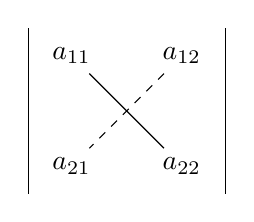
\begin{tikzpicture}
  \draw (-1.25,1.05) -- (-1.25,-1.05);

  \node at (-.7,.7) (a11) {$a_{11}$};
  \node at (.7,-.7) (a22) {$a_{22}$};
  \draw (a11) -- (a22);

  \node at (.7,.7) (a12) {$a_{12}$};
  \node at (-.7,-.7) (a21) {$a_{21}$};
  \draw[dashed] (a12) -- (a21);

  \draw (1.25,1.05) -- (1.25,-1.05);
\end{tikzpicture}

  \caption{对角线法则}
  \label{图:二阶对角线法则}
\end{figure}

\subsubsection{二元线性方程组的解}
\paragraph{}
利用二阶行列式的概念和对角线法则,\eqref{二元线性方程组的解}式中$x_1,x_2$的分子也可写成二阶行列式,即
\begin{equation*}
  b_1a_{22} - a_{12}b_2 = \left|\begin{array}{ll} b_1 & a_{12} \\ b_2 & a_{22}\end{array}\right|, \;
  a_{11}b_2 - b_1a_{21} = \left|\begin{array}{ll} a_{11} & b_1 \\ a_{21} & b_2\end{array}\right|,
\end{equation*}

\paragraph{}
若记
\begin{equation*}
  D = \left|\begin{array}{ll} a_{11} & a_{12} \\ a_{21} & a_{22} \end{array}\right|, \;
  D_1 = \left|\begin{array}{ll} b_1 & a_{12} \\ b_2 & a_{22} \end{array}\right|, \;
  D_2 = \left|\begin{array}{ll} a_{11} & b_1 \\ a_{21} & b_2 \end{array}\right|, \;
\end{equation*}
那么\eqref{二元线性方程组的解}式可写成
\begin{equation*}
  x_1 = \frac{D_1}{D} = \frac{\left|\begin{array}{ll} b_1 & a_{12} \\ b_2 & a_{22} \end{array}\right|}{\left|\begin{array}{ll} a_{11} & a_{12} \\ a_{21} & a_{22} \end{array}\right|}, \;
  x_2 = \frac{D_2}{D} = \frac{\left|\begin{array}{ll} a_{11} & b_1 \\ a_{21} & b_2 \end{array}\right|}{\left|\begin{array}{ll} a_{11} & a_{12} \\ a_{21} & a_{22} \end{array}\right|}.
\end{equation*}

\paragraph{}
注意,这里的分母$D$是由方程组\eqref{消元法解二元线性方程组}的系数所确定的二阶行列式(称系数行列式),$x_1$的分子$D_1$是常数项$b_1,b_2$替换$D$中$x_1$的系数$a_{11}, a_{21}$(第$1$列)所得的二阶行列式;$x_2$的分子$D_2$是用常数项$b_1, b_2$替换$D$中$x_2$的系数$a_{12}, a_{22}$(第$2$列)所得的二阶行列式。

\subsection{三阶行列式}
\subsubsection{定义}
\paragraph{}
\textbf{定义~~}设有$9$个数排成$3$行$3$列的数表
\begin{equation}
  \label{三阶数表}
  \begin{array}{lll}
    a_{11} & a_{12} & a_{13} \\
    a_{21} & a_{22} & a_{23} \\
    a_{31} & a_{32} & a_{33},
  \end{array}
\end{equation}
记
\begin{align}
\centering
  \begin{split}
    \label{三阶行列式}
    &\;\left|\begin{array}{lll}
      a_{11} & a_{12} & a_{13} \\
      a_{21} & a_{22} & a_{23} \\
      a_{31} & a_{32} & a_{33}
    \end{array}\right| \\
    =&\; a_{11}a_{22}a_{33} + a_{12}a_{23}a_{31} + a_{13}a_{21}a_{32} - \\
    &\; a_{11}a_{23}a_{32} - a_{12}a_{21}a_{33} - a_{13}a_{22}a_{31},
  \end{split}
\end{align}
\eqref{三阶行列式}称为数表\eqref{三阶数表}所确定的三阶行列式。

\subsubsection{对角线法则}
\begin{figure}[H]
\centering
  % 三阶行列式的对角线法则
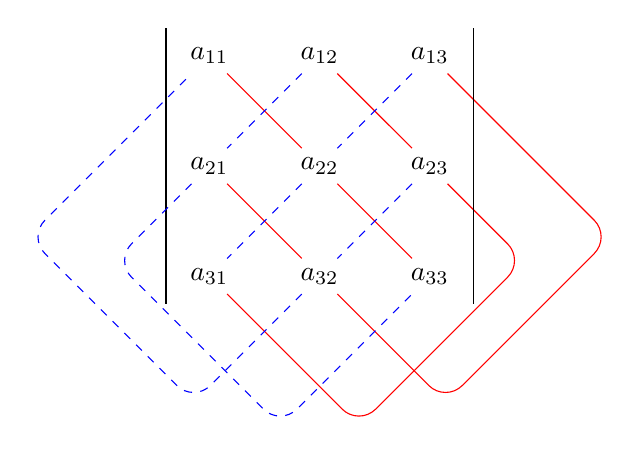
\begin{tikzpicture}

  \draw (-1.95,1.75) -- (-1.95,-1.75);

  \node at (-1.4,1.4) (a11) {$a_{11}$};
  \node at (0,1.4) (a12) {$a_{12}$};
  \node at (1.4,1.4) (a13) {$a_{13}$};

  \node at (-1.4,0) (a21) {$a_{21}$};
  \node at (0,0) (a22) {$a_{22}$};
  \node at (1.4,0) (a23) {$a_{23}$};

  \node at (-1.4,-1.4) (a31) {$a_{31}$};
  \node at (0,-1.4) (a32) {$a_{32}$};
  \node at (1.4,-1.4) (a33) {$a_{33}$};

  \draw[red] (a11) -- (a22) -- (a33);
  \draw[red,rounded corners=3mm] (a12) -- (a23) -- (2.6,-1.2) -- (0.5,-3.3) -- (a31);
  \draw[red,rounded corners=3mm] (a21) -- (a32) -- (1.6,-3) -- (3.7,-0.9) -- (a13);

  \draw[dashed,blue] (a13) -- (a22) -- (a31);
  \draw[dashed,blue,rounded corners=3mm] (a12) -- (a21) -- (-2.6,-1.2) -- (-0.5,-3.3) -- (a33);
  \draw[dashed,blue,rounded corners=3mm] (a23) -- (a32) -- (-1.6,-3) -- (-3.7,-0.9) -- (a11);

  \draw (1.95,1.75) -- (1.95,-1.75);
\end{tikzpicture}

  \caption{对角线法则}
  \label{图:三阶对角线法则}
\end{figure}

\paragraph{}
对角线法则只适用于二阶与三阶行列式,下面先介绍全排列及其逆序数,然后由此引出$n$阶行列式的概念。

\subsection{全排列及其逆序数}
\subsubsection{全排列}
\paragraph{}
把$n$个不同的元素排成一列,叫做这$n$个元素的\textbf{全排列}(简称\textbf{排列})。

\paragraph{}
从$n$个元素中任取一个放在第一个位置上,有$n$种取法;又从剩下的$n-1$个元素中任取一个放在第二个位置上,有$n-1$种取法;依此类推,于是:
\begin{equation*}
  P_n = n \bigcdot (n-1) \bigcdot \cdots \bigcdot 3 \bigcdot 2 \bigcdot 1 = n!.
\end{equation*}

\subsubsection{逆序数}
\paragraph{}
概念:
\begin{enumerate}
  \item \textbf{标准次序}:$n$个不同的自然数,按由小到大的顺序排序
  \item \textbf{逆序}:当某两个元素的先后次序与标准次序不同时,就说有$1$个\uwave{逆序}
  \item \textbf{排列的逆序数}:一个排列中所有逆序的总数
  \item \textbf{奇/偶排列}:逆序数为奇/偶数
\end{enumerate}

\paragraph{}
下面讨论计算排列的逆序数的方法:

\paragraph{}
一般性,设$n$个元素为$1$至$n$这$n$个自然数,并规定由小到大为标准次序,设:
\begin{equation*}
  p_1p_2\cdots p_n
\end{equation*}
为这$n$个自然数的一个排列,考虑元素$p_i(i=1,2,\cdots,n)$,如果比$p_i$大的且排在$p_i$前面的元素有$t_i$个,就说$p_i$这个元素的逆序数是$t_i$。全体元素的逆序数之总和
\begin{equation*}
  t = t_1 + t_2 + \cdots + t_n = \sum_{t=1}^n t_i,
\end{equation*}
即是这个排列的逆序数。

\subsection{$n$阶行列式的定义}

\subsection{对换}

\subsection{行列式的性质}

\subsection{行列式按行(列)展开}

\subsection{克拉默法则}
